\documentclass[graybox]{svmult}

\usepackage{mathptmx}
\usepackage{helvet}
\usepackage{courier}
\usepackage{type1cm}
\usepackage{makeidx}
\usepackage{graphicx}
\usepackage{multicol}
\usepackage[bottom]{footmisc}
\usepackage{placeins}
\usepackage{listings}
\usepackage{xcolor}
\definecolor{very-light-gray}{gray}{0.95}

\makeindex

\begin{document}

\title*{Genetic Algorithm Based Formula Generation for Curve Fitting in Time Series Forecasting Implemented as Mobile Distributed Computing}
\titlerunning{GA Formula Generation for CF in TSF Implemented as MDC}

\author{Rumen Ketipov, Georgi Kostadinov, Plamen Petrov,  \\ Iliyan Zankinski, Todor Balabanov\textsuperscript{0000-0003-3139-069X}}
\authorrunning{R. Ketipov et al.}

\institute{
	Rumen Ketipov \email{rketipov@iit.bas.bg}
\and 
	Georgi Kostadinov \email{g.kostadinov@iit.bas.bg}
\and 
	Plamen Petrov \email{p.petrov@iit.bas.bg}
\and 
	Iliyan Zankinski \email{iliyan@hsi.iccs.bas.bg}
\and 
	Todor Balabanov \email{todorb@iinf.bas.bg} 
\at 
	Institute of Information and Communication Technologies - Bulgarian Academy of Sciences, acad. Georgi Bonchev Str, block 2, 1113 Sofia, Bulgaria}

\maketitle

\abstract*{Times series forecasting has many important real life applications. Such forecasting is widely used in statistics, signal processing, pattern recognition, econometrics, mathematical finance, weather forecasting, earthquake prediction, electroencephalography, control engineering, astronomy, communications engineering and in any applied mathematics field where temporal measurements are done. 
\vskip 0.01em
In last few decades time series forecasting receives a lot of attention from the researchers in the machine learning domain. Many different forecasting models are developed with the usage of different prediction approaches. Artificial neural networks are a bright example of such forecasting technique. The main goal is learning of data dependency between past and future values of the time series when artificial neural network is used. If the weights of the artificial neural networks are taken as coefficients of a complex polynomial the forecasting can be presented as curve fitting problem. 
\vskip 0.01em
This research proposes forecasting approach a little bit different than the approach used in the artificial neural networks. Set of mathematical formulas are presented as expression trees in a genetic algorithm population. The goal in this genetic algorithm based optimization is searching of a mathematical expression which can provide the best curve fitting formula according time series values. Because of the genetic algorithms' extremely high degree of parallelism possibilities calculations in this research are organized as distributed computing solutions on a mobile devices with Android operating system.}

\abstract{Times series forecasting has many important real life applications. Such forecasting is widely used in statistics, signal processing, pattern recognition, econometrics, mathematical finance, weather forecasting, earthquake prediction, electroencephalography, control engineering, astronomy, communications engineering and in any applied mathematics field where temporal measurements are done. 
\vskip 0.01em
In last few decades time series forecasting receives a lot of attention from the researchers in the machine learning domain. Many different forecasting models are developed with the usage of different prediction approaches. Artificial neural networks are a bright example of such forecasting technique. The main goal is learning of data dependency between past and future values of the time series when artificial neural network is used. If the weights of the artificial neural networks are taken as coefficients of a complex polynomial the forecasting can be presented as curve fitting problem. 
\vskip 0.01em
This research proposes forecasting approach a little bit different than the approach used in the artificial neural networks. Set of mathematical formulas are presented as expression trees in a genetic algorithm population. The goal in this genetic algorithm based optimization is searching of a mathematical expression which can provide the best curve fitting formula according time series values. Because of the genetic algorithms' extremely high degree of parallelism possibilities calculations in this research are organized as distributed computing solutions on a mobile devices with Android operating system.}

\section{Introduction} \label{Introduction}

This research focuses on the capabilities distributed genetic algorithms to be used for mathematical formulas generation as tool for time series curve fitting. Each of the components used in this research will be introduced in the following subsections. 

\subsection{Time Series} \label{Time Series}

Financial time series forecasting is an area of high researchers interest \cite{nava01} from many decades. Having an accurate forecast in the financial world is crucial for many important decision makings \cite{catania01}. Time series are ordered measurements of particular variable done in a temporal manner \cite{chen01}. In most cases values are measured on equal intervals, but it is not a mandatory condition. Time series analysis is applicable in processes with clear repetition pattern \cite{mueen01}. Measurements done in a temporal order are presented as points in a two-dimensional space. For visualization purposes in many cases these points are connected with straight lines, which is a simplified form of linear interpolation for the values between two neighboring measurements. With such organization of points in two-dimensional space many different curves can be proposed for some generalization of the data nature (curve fitting problem). Linear regression for example can be used for trend estimation. In this case parameters of line equation are calculated such as that this line is the closest line for the given points. Another much more complicated generalization can be the Lagrange polynomial. In this case the parameters of a polynomial of lowest degree that assumes at each value from X the corresponding value on Y (curve coincide at each point) are estimated. Theoretically infinite number of curves can satisfy the condition to pass across finite number of points in two-dimensional space. In the same context if calculations done in an artificial neural network are evaluated as mathematical expression it will give rough descsription of an equation in two-dimensional space. The general advantage of artificial neural networks is that they are capable to self-adjust coefficients \cite{aljarah01} in this equation. In some cases the optimization inside the artificial neural network is done by genetic algorithm \cite{zhang01,kapanova01}. For this study it is much more interesting how genetic algorithms can be used for curve fitting as self-adaptive system similar to the artificial neural networks. 

\subsection{Genetic Algorithms} \label{Genetic Algorithms}

Genetic algorithms are metaheuristic for global optimization inspired by the natural processes in the biological evolution. Genetic algorithms are population based \cite{mirjalili01} and they are subset of a larger class algorithms called evolutionary algorithms \cite{liu01}. Searching for a solution with genetic algorithms is based on three general operations - selection, crossover and mutation applied over population with individuals. Each individual is a vector into the solutions space. 

Solving a problem starts with proper encoding of the individuals. There are many different encoding possibilities like binary encoding, integer numbers encoding, real numbers encoding, permutation encoding and etc. One less popular encoding is the expression tree encoding. In this case the individuals are represented with tree as data structure. Each node of the tree is a mathematical operation, on each leaf of the tree is an expression operand. 

The process of the selection is related to pickup of two parents, which will be recombined for the creation of the new generation. There are many ways for the selection to be done. The most popular are - roulette wheel selection, rank selection, steady-state selection and etc. The process of parents selection is important, because it is expected that better parents have better chances to produce better children. During the selection process individuals with higher survival capabilities (fitness value) have better chances to mate. In the same time individuals with worse survival capabilities should also have some chances to mate. In some implementations of genetic algorithms elitism rule is applied. This means that the best found solutions are not removed from the population and this individuals have much higher chances and options to mate. 

Crossover operation gives to the algorithm exploration capabilities and it is very dependent of the individuals encoding. In most of the cases crossover is done by single cut, two points cut or uniform merge. The main idea for the crossover is that two parents are exchanging different parts in order new individual to be created. When single cut point is applied parents are divided on two parts and second half of the parents are swapped. The place of the cut point is chosen randomly. For expression tree encoding single cut crossover is almost intuitive choice. Branches (sub-trees) in both parents are randomly selected and swapped. 

Mutation operation gives to the algorithm exploitation capabilities and it is also very dependent of the individuals encoding. During mutation only small part of the individual is changed. In the simplest form only a single bit is inverted. With integer or real numbers small delta is added or subtracted. When permutations are encoded two elements are exchanged for achieving mutation. With expression tree encoding few mutations are possible - random change of mathematical operation in the randomly selected node, random change of the operand in randomly selected leaf, random swap of nodes and etc. 

After creation of the new generation each individual is evaluated and fitness value is assigned. The individuals from the old generation and the new generation are sorted according their fitness values and second half of the list is removed from the population. The fitness function used for individuals evaluation is extremely problem dependent. 

Genetic algorithms have a group of parameters like - population size (usually estimated experimentally), crossover rate (in most cases 0.95 is advisable), mutation rate (in most cases 0.1 or 0.05 is advisable), elitism flag and etc. There is no general theory about population size and because of this the only applicable way for estimation of this parameters is by trying different possibilities. The crossover rate shows the chance a child to be produced by exchanging parts of the parents. When this parameter is less than one it means that there would be chances some parents to skip crossover procedure and to bypass directly to mutation procedure. Mutation rate shows the chance of every single element in the particular individual to be changed. When the mutation rate is very low few neighboring solutions are checked and the chances to approach global optimum are lower. 

The organization of genetic algorithms computation by presence of population and operators applied over this population makes genetic algorithms perfect for parallel computations \cite{cheng01}. In distributed computing system genetic algorithm global population is used (client-server architecture) and many local sub-populations are evolved without real need for information exchange between territorial separated computers. 

\subsection{Distributed Computing} \label{Distributed Computing}

Distributed computing is a computational organization in a system where components are located on different networked computers \cite{balabanov01}. These computers communicates and coordinates their activities by passing messages between each other. Distributed computing is remarkable with: concurrency of components, lack of a global clock, and independent failure of components. In distributed computing, a problem is divided into many tasks, each of which is solved by one or more computers \cite{godfrey01}, which communicate with each other via message passing \cite{andrews01}. Distributed computing is generally used for solving a large computational problems. 

In this study for distributed computing will be accepted the definition which states that each processor has its own memory and it is embedded in separate device. Under this conditions calculating instructions run in parallel, which is the only relation with the parallel computing. The system is tolerant to a single component failure. The exact structure of the system is not know in advance and it changes with the time passing, because some nodes get in when some nodes get out \cite{balabanov02}. The whole system consists of heterogeneous hardware and variety types of network connectivity. 

When end users donate their computational resources it is called donated distributed computing and in most cases computations are organized as screensaver applications or low consumption demon processes. Many devices around the world have periods of idle usage. In such cases their owners are capable to donate this calculating power. Donated calculating power is mainly used for low budget projects usually in society help. Many scientific projects are organized around donated distributed computing and the most popular of them is SETI@home, which analyzes radio signals from the deep space. 

Last decade was marked with huge progress of mobile devices and communications, which gave to the scientist new capabilities for implementation of distributed computing software implementation. For example modern mobile devices are capable to provide active wallpapers instead of screensavers. Another option are the widgets supported in the modern mobile operating systems. But the best advantage of the mobile distributed computing is that most of the devices are operating 24/7, which is not the case with the desktop computers and working stations. 

\section{Proposed Solution} \label{Proposed Solution}

There are different ways in which arithmetic expressions can be presented into the computer memory. One of the most used representations is an expression tree. Such representation is convenient in many cases, but for the current research arithmetic expressions are encoded as simple text strings. The crossover operator in this case is simple single cut and swap. Mutation is organized as random change of a mathematical operator, random change of a mathematical function and random change of a operand. 

\begin{lstlisting}[caption={Genetic algorithm pseudo-code.},label={lst01},backgroundcolor=\color{very-light-gray},frame={single}]
begin
  t = 0;
  initialize P(t);
  evaluate structures in P(t);
  while termination condition not satisfied do
  begin
    t = t + 1;
    select_repro C(t) from P(t-1);
    recombine and mutate structures in C(t)
    forming C’(t);
    evaluate structures in C’(t);
    select_replace P(t) from C’(t) and P(t-1);
  end
end
\end{lstlisting}
\FloatBarrier

For the genetic algorithm a classical implementation is proposed (Listing \ref{lst01}) as described in \cite{baeck01}.

\section{Experiments} \label{Experiments}

Experiments are done as Android mobile application. On the client side Apache Commons Genetic Algorithms Framework \cite{apache01} is used with the parameters listed in Tab. \ref{tab01}. Mathematical expressions are presented and evaluated with Java build of mXparser \cite{gromada01} software library. On the server side PHP/MySQL based solution \cite{balabanov03} is responsible for synchronization and financial time series data supply. 

\begin{figure}[b]
\sidecaption
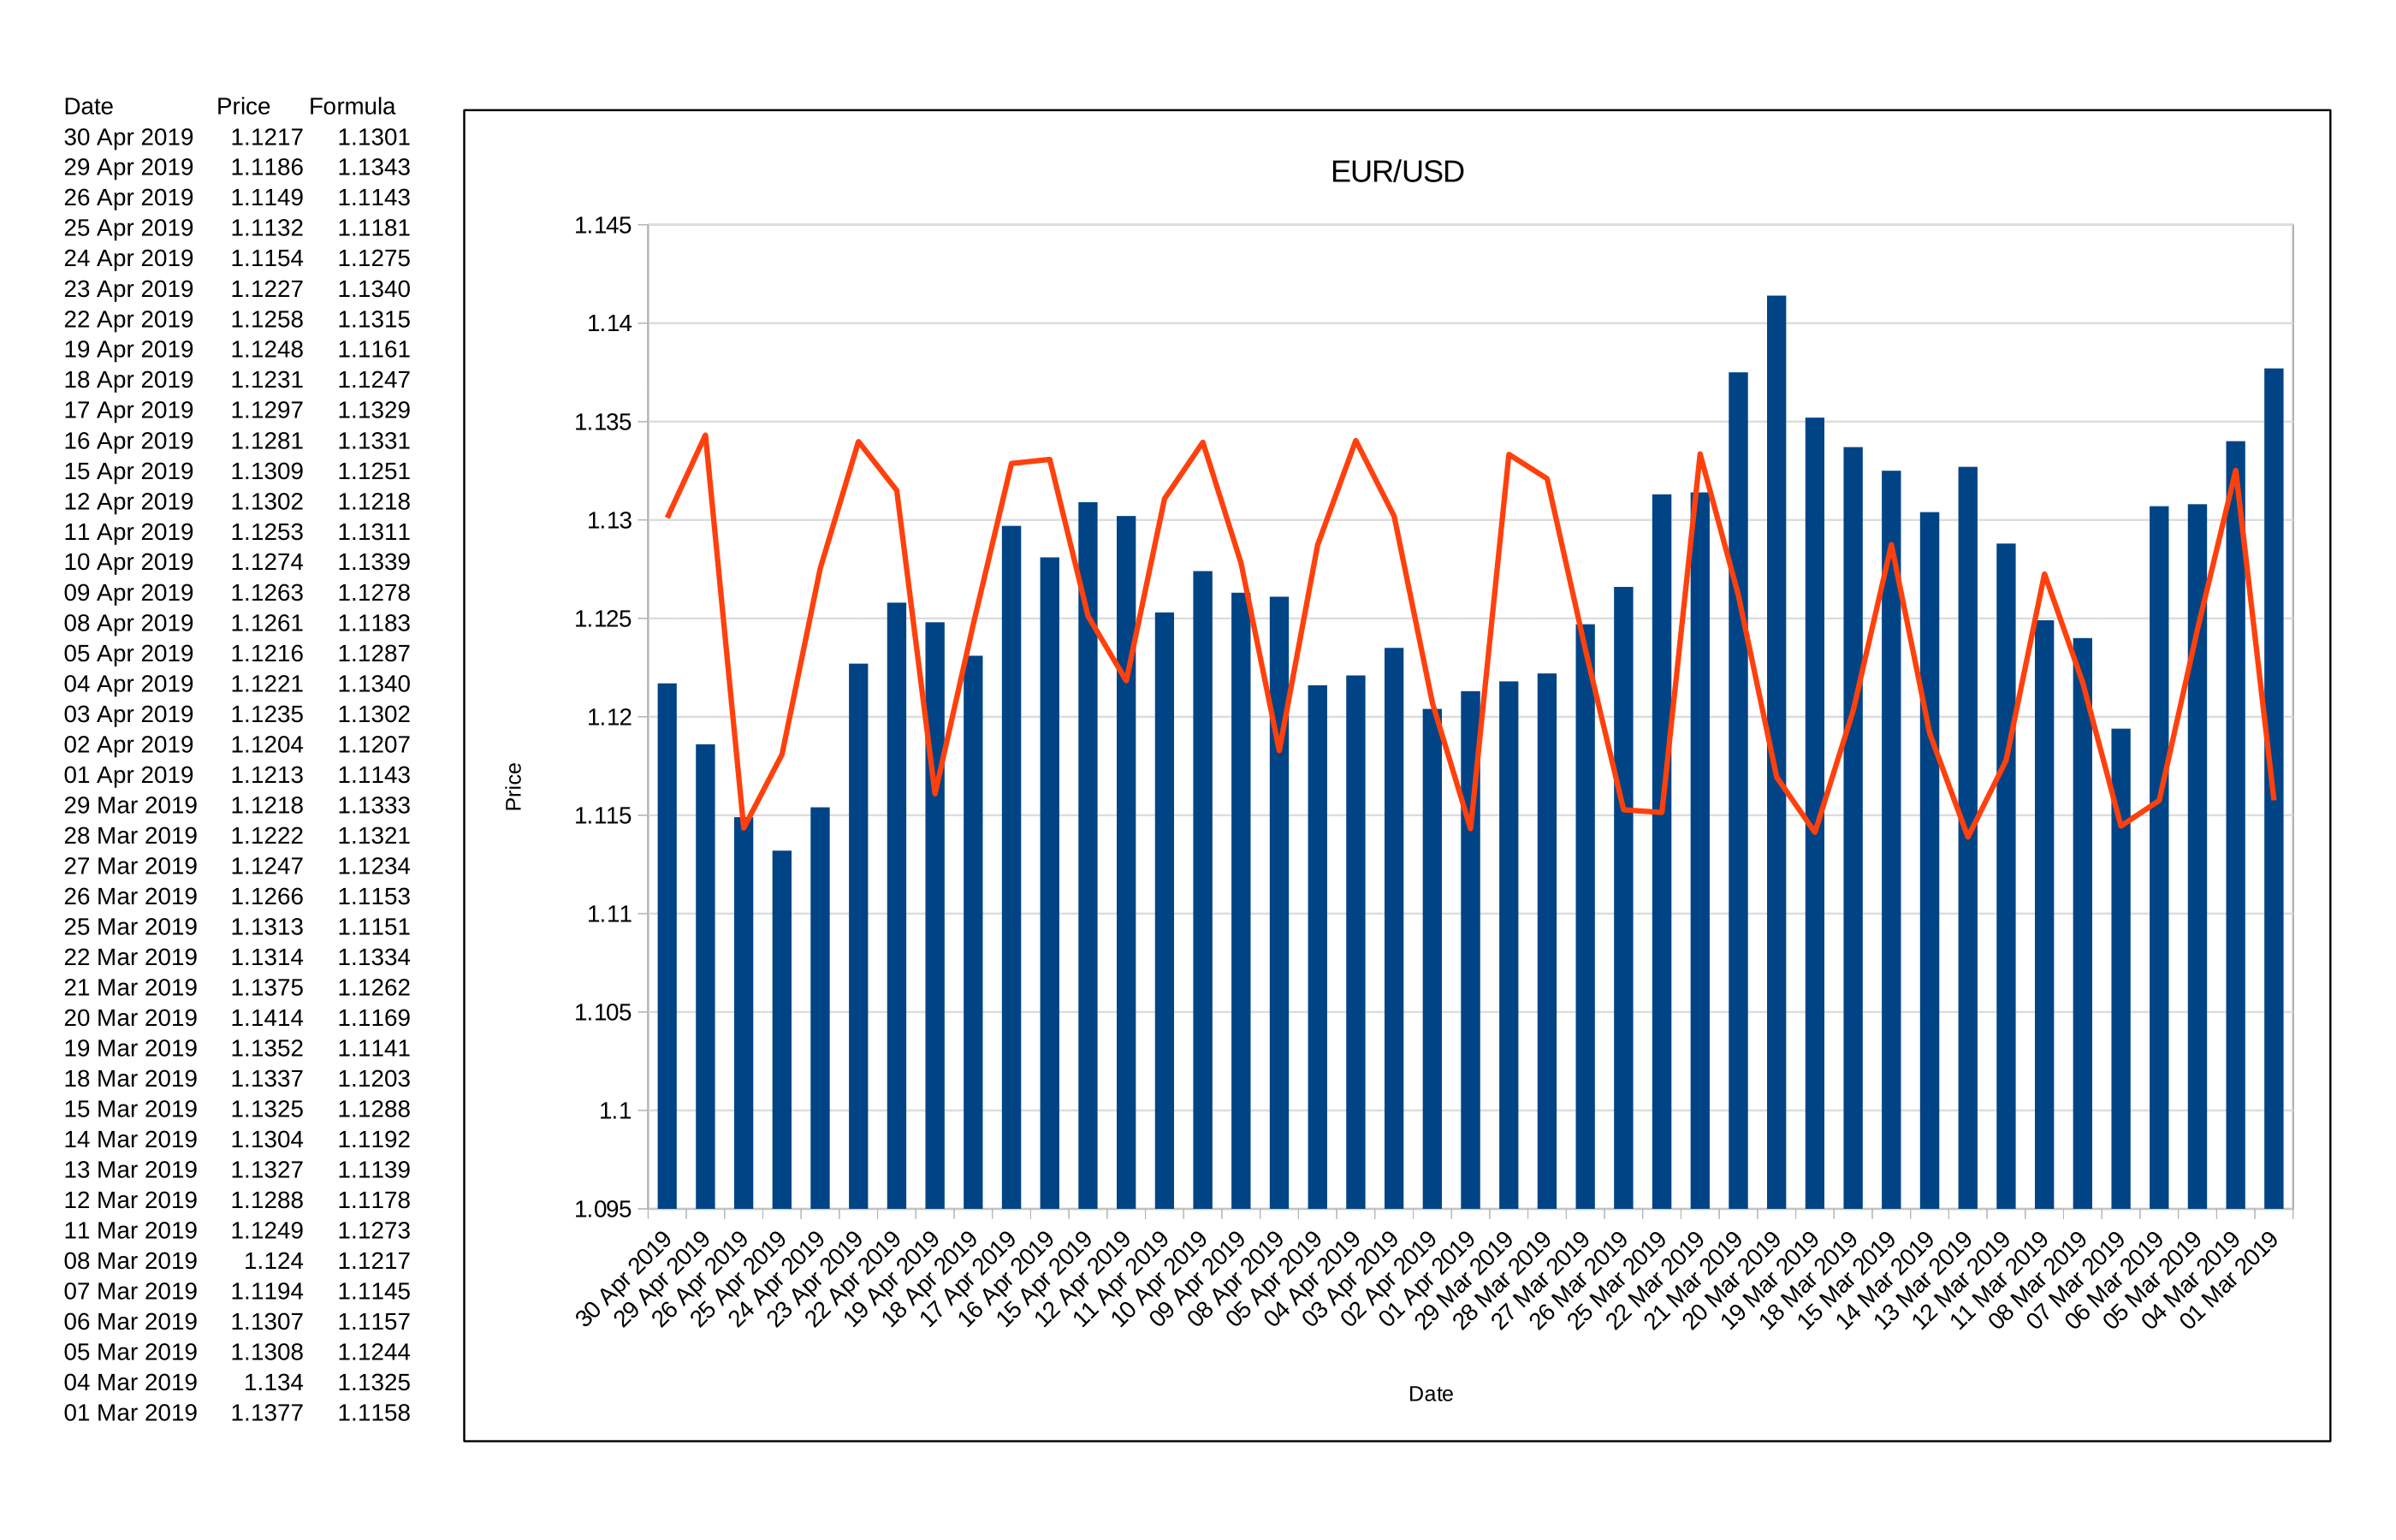
\includegraphics[scale=0.12]{fig01.png}
\caption{EUR/USD rate for two months.}
\label{fig01}
\end{figure}
\FloatBarrier

Publicly available data are used for EUR/USD rate for two months in 2019 year (Fig. \ref{fig01}). Bars in the chart shows the real world price. The line above the bars is the line of the formula generated by the proposed genetic algorithm. The approximation of the price values follows the shape of the bars. 

\begin{table}
\caption{Genetic algorithm parameters.}
\label{tab01}
\begin{tabular}{p{6.9cm}p{4.4cm}}
\hline\noalign{\smallskip}
\textbf{Parameter} & \textbf{Value} \\
\noalign{\smallskip}\svhline\noalign{\smallskip}
generation gap & 0.97 \\
crossover rate & 0.95 \\
mutation rate & 0.03 \\
maximum generations & 100 \\
number of individuals & 37 \\
number of variables & floating \\
inserted rate & 100 \% \\
\noalign{\smallskip}\hline\noalign{\smallskip}
\end{tabular}
\end{table}
\FloatBarrier

In 100 generations the genetic algorithm proposes a solution presented with the formula in Eq. \ref{equ01}.

\begin{equation}\label{equ01}
price = 0.485 + 0.01 * sin(day - 2.3) + log(day / 10000)
\end{equation}

The equation has few terms with sine and logarithmic functions used. The input of the equation is time value (number of days). The output of the equation is a prediction of the EUR/USD rate. 

\section{Conclusions} \label{Conclusions}

This research shows that genetic algorithms are a promising approach for financial time series forecasting, when they are used for formula generated predictors. The nature of genetic algorithms allows extremely high degree of parallel computations. This fact allows creation of very efficient distributed computing systems even on modern mobile devices. 

As future research it will be interesting different communication capabilities to be investigated as described in \cite{alexandrov01} in order better genetic algorithms indivuduals exchange to be achieved. Also it will be interesting generalized artificial neural networks \cite{tashev01} to be tested in combination with genetic algorithms formula generation.

\begin{acknowledgement}
This work was funded by Velbazhd Software LLC.
\end{acknowledgement}

\begin{thebibliography}{99}

\bibitem{nava01} Nava, N., Di Matteo, T., Aste, T., \textbf{\textit{Financial Time Series Forecasting Using Empirical Mode Decomposition and Support Vector Regression}}, RISKS, \textbf{6}(1), article 7, 2018.

\bibitem{catania01} Catania L., Grassi S., Ravazzolo F., \textbf{\textit{Predicting the Volatility of Cryptocurrency Time-Series}}, Mathematical and Statistical Methods for Actuarial Sciences and Finance, Springer, Cham, p. 203--207, 2018.

\bibitem{chen01} Chen, J., Boccelli, DL., \textbf{\textit{Real-time forecasting and visualization toolkit for multi-seasonal time series}}, Environmental Modelling \& Software, \textbf{105}, p. 244--256, 2018.

\bibitem{mueen01} Mueen, A., Keogh, E., Zhu, Q., Cash, S., Westover, B., \textbf{\textit{Exact Discovery of Time Series Motifs}}, Proceedings of the SIAM International Conference on Data Mining, p. 473--484, 2009.

\bibitem{aljarah01} Aljarah, I., Faris, H., Mirjalili, S., \textbf{\textit{Optimizing connection weights in neural networks using the whale optimization algorithm}}, Soft Computing, Springer Berlin Heidelberg, \textbf{22}(1), p. 1--15, 2016.

\bibitem{zhang01} Zhang, R., Tao, J., \textbf{\textit{A Nonlinear Fuzzy Neural Network Modeling Approach Using an Improved Genetic Algorithm}}, IEEE Transactions on Industrial Electronics, \textbf{65}(7), p. 5882--5892, 2018.

\bibitem{kapanova01} Kapanova, K., Dimov, I., Sellier, J.M., \textbf{\textit{A genetic approach to automatic neural network architecture optimization}}, Neural Computing and Applications, Springer London, \textbf{29}(5), p. 1481--1492, 2016.

\bibitem{mirjalili01} Mirjalili S., \textbf{\textit{Genetic Algorithm}}, Evolutionary Algorithms and Neural Networks. Studies in Computational Intelligence, Springer, Cham, \textbf{780}, p. 43--55, 2019.

\bibitem{liu01} Liu, J., Abbass, H.A., Tan, K.C., \textbf{\textit{Evolutionary Computation}}, Evolutionary Computation and Complex Networks, Springer, Cham, p. 3--22, 2019.

\bibitem{cheng01} Cheng, JR., Gen, M., \textbf{\textit{Accelerating genetic algorithms with GPU computing: A selective overview}}, Computers \& Industrial Engineering, Elsevier, \textbf{128}, p. 514--525, 2019.

\bibitem{balabanov01} Balabanov, T., Genova, K., \textbf{\textit{Distributed System for Artificial Neural Networks Training Based on Mobile Devices}}, Proceedings of International Conference AUTOMATICS AND INFORMATICS, Federation of the Scientific Engineering Unions John Atanasoff Society of Automatics and Informatics, p. 49--52, 2016.

\bibitem{godfrey01} Godfrey, B., \textbf{\textit{A primer on distributed computing}}, http://billpg.com/bacchae-co-uk/docs/dist.html Last visited: 01-May-2019 16:07:00 EET, 2006.

\bibitem{andrews01} Andrews, G., \textbf{\textit{Foundations of Multithreaded, Parallel, and Distributed Programming}}, Addison–Wesley, p. 291--292, 2000.

\bibitem{balabanov02} Balabanov, T., Zankinski, I., Barova, M., \textbf{\textit{Strategy for Individuals Distribution by Incident Nodes Participation in Star Topology of Distributed Evolutionary Algorithms}}, Cybernetics and Information Technologies, \textbf{16}(1), p. 80--88, 2016.

\bibitem{baeck01} Baeck, T., Fogel, DB., Michalewicz, Z., \textbf{\textit{Evolutionary Computation 1 - Basic Algorithms and Operators}}, Institute of Physics Publishing - Bristol and Philadelphia, p. 65--68, 2000.

\bibitem{apache01} \textbf{\textit{Apache Commons Genetic Algorithms Framework}}, http://commons.apache.org/proper/commons-math/userguide/genetics.html Last visited: 12-May-2019 12:36:56 EET, 2016.

\bibitem{gromada01} Gromada, M., \textbf{\textit{mXparser - Math Expression Evaluator / Parser - Library}}, http://www.mathparser.org/ Last visited: 12-May-2019 12:44:12 EET.

\bibitem{balabanov03} Balabanov, T., \textbf{\textit{Distributed System for Time Series Prediction with Evolutionary Algorithms and Artificial Neural Networks}}, Abstracts of Dissertations - Institute of Information and Communication Technologies - Bulgarian Academy of Sciences, \textbf{6}, 2017.

\bibitem{alexandrov01} Alexandrov, A., \textbf{\textit{Comparative analysis of IEEE 802.15.4 based communication protocols used in wireless intelligent sensor systems}}, Proceedings of the International conference RAM, p. 51--54, 2014.

\bibitem{tashev01} Tashev, T., Hristov, H., \textbf{\textit{Modeling of synthesis of information processes with generalized nets}}, Cybernetics and Information Technologies, \textbf{3}(2), p. 92--104, 2003.

\end{thebibliography}

\end{document}
